\documentclass[a4paper]{article}

\usepackage[english]{babel}
\usepackage[utf8]{inputenc}
\usepackage{amsmath,amssymb}
\usepackage{gensymb}
\usepackage{graphicx}
\usepackage{comment}
%\usepackage[colorinlistoftodos]{todonotes}
\usepackage{float}
\usepackage[left=2cm,right=2cm,bottom=2cm,includefoot]{geometry} % pour les marges
%\usepackage{sidecap} % pour avoir des titres de fig/table sur les côtés
%\usepackage{anyfontsize}
\usepackage{hyperref}
\hypersetup{
    colorlinks   = true, % Colours links instead of ugly boxes
    urlcolor     = blue, % Colour for external hyperlinks
    linkcolor    = blue,% Colour of internal links
    citecolor    = blue   % Colour of citations
}
\usepackage[x11names]{xcolor}
%\usepackage{subfigure}
%\usepackage{listingsutf8}
\usepackage{listings} % pour insérer les codes
%\usepackage{textcomp}
%\usepackage{enumerate}
%\usepackage{multicols}
\usepackage{xspace}
\usepackage{caption}
%\usepackage{titlesec} % pour pouvoir modifier les titres des sections
\usepackage[bottom]{footmisc} % pour que les notes en bas de page colle le bas même si page vide
\usepackage[normalem]{ulem} % pour pouvoir barrer un texte quelconque
%\usepackage{clrscode3e} % pour les pseudo-codes
%\usepackage{tikz} % pour les arbres
\usepackage{tablefootnote} % Footnote in table -> use \tablefootnote{}
%\usepackage[nomessages]{fp} % see https://tex.stackexchange.com/questions/154224/fp-calculation-variable
\usepackage{diagbox}

%\renewcommand{\thesubsection}{\thesection.\alph{subsection}}
\newcommand{\eme}{$^{\text{ème}}$\xspace}
\newcommand{\rem}[1]{\textcolor{red}{[#1]}}
\newcommand{\para}[1]{\paragraph{#1}\quad\\}
\newcommand{\vsp}{\vspace{1em}}
\newcommand{\ds}{\displaystyle}
\renewcommand{\tt}[1]{\texttt{#1}\xspace}
\renewcommand{\u}[1]{\underline{#1}\xspace}
\newcommand{\ie}{\textit{i.e.}\xspace}
\renewcommand{\b}{$\bullet$\xspace}
\newcommand{\itemb}{\item[\b]}
\colorlet{mygreen}{green!60!black}
\newcommand{\newRem}[2]{\expandafter\newcommand\csname#1\endcsname[1]{\textcolor{#2}{[#1: ##1]}}}
\newRem{nico}{mygreen}
\newRem{remi}{blue}

%\newcommand{\ordi}[1]{\hyperref[ax:#1]{\includegraphics[scale=0.004]{ordi}}\\}
\newcommand{\code}[1]{\begin{minipage}{\textwidth}\lstinputlisting[label=ax:#1,title=$\mathtt{#1.m}$]{MatLab_codes/#1.m}\end{minipage}}
\lstset{
    inputencoding=utf8,  
    extendedchars=true,
    language=C,
    frame=single,
    breaklines=true,
    numbers=left,
    numbersep=5pt,
    basicstyle=\footnotesize\ttfamily,
    commentstyle=\itshape\color{gray},
    keywordstyle=\bf\color{mygreen},
    %identifierstyle=\color{black},
    %stringstyle=\color{black},
    %numberstyle=\color{red},
    %emph={read2Darrayshm,write2Darrayshm,send_message,read_message,writeshm,readshm,wait,waitAll,signal,signalAll},
    %emphstyle=\color{orange!70!red},
    morekeywords={foreach, interrupt},
    morecomment=[l][\itshape]{!!},
    showstringspaces=false,
    float,
    floatplacement=H,
    literate=%
        {à}{{\`a}}1
        {é}{{\'e}}1
        {è}{{\`e}}1
        {É}{{\'E}}1
        {î}{{\^i}}1
        {ô}{{\^o}}1
        {‰}{{\textperthousand}}1
        {µ}{{$\mu$}}1
}

\setlength{\parindent}{0cm}

\usepackage{apacite}
\usepackage{algorithm}
\usepackage{algorithmic}

\begin{document}
\thispagestyle{empty}
\setcounter{page}{0}
\begin{center}
    \begin{tabular}{c}
        \begin{minipage}{.95\textwidth}
            \centering
            \begin{minipage}{0.65\textwidth}
                \vspace{0.8cm}
                \textsc{\LARGE Master 1 Electrical Engineering}\\
                \quad\\
                \quad\\
                \textsc{\Large Academic Year 2019-2020}\\   
            \end{minipage}\hspace{\stretch{1}}
            \begin{minipage}{0.23\textwidth}
                \begin{figure}[H]
                
\includegraphics[scale=0.1]{logo_unif}
                \end{figure}
            \end{minipage}
        \end{minipage}
        
        \vspace{1.5cm}\\
        
        \hline
        \\
        \begin{minipage}{.9\textwidth}
            \scshape\LARGE
            \centering
            INFO8003-1 - Optimal decision making\\
            {\large project - Inverted Double Pendulum : Searching
                    High-Quality Policies to Control an
                    Unstable Physical System.}
        \end{minipage}\\
        \\
        \hline
        \vspace{1.5cm}\\
        
        \begin{minipage}{10cm}
            \Large\sffamily\centering
            %\begin{flushleft}
            Nicolas MAHIAT (s160703)\\
            Rémi RAIMONDI (s162464)\\
            %\end{flushleft}        
        \end{minipage}
    \end{tabular}

    \vspace{1cm}
    \vfill
    \begin{figure}[H]
        \centering
        %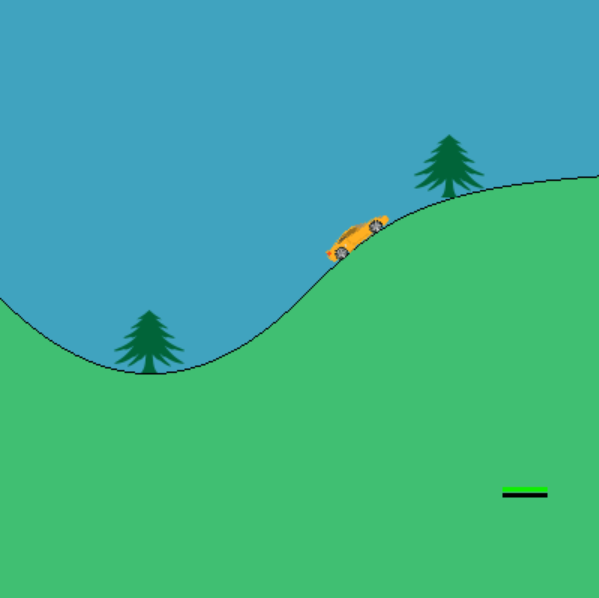
\includegraphics[width=.7\textwidth]{pagedegarde.png}
    \end{figure}
    \vfill
\end{center}

\section{Domain}

\paragraph{State space:} The state space for this control problem is $\{(x, \Dot{x}, \theta, \Dot{\theta}, \gamma, \Dot{\gamma}) \in \mathbb{R}^6|x \in ]-\infty, +\infty[$\} plus a terminal state. $x$, $\theta$, and $\gamma$ are respectively the horizontal position of the center of the cart, the angle between the first pole and the upright direction taken at the center of the cart and the angle between the second pole and the upright direction taken at the center of the first pole. While $\Dot{x}$, $\Dot{\theta}$, $\Dot{\gamma}$ correspond respectively to the horizontal velocity of the cart, the angular velocity of the angle $\theta$ and the angular velocity of the angle $\gamma$. A terminal state is reached when the vertical position of the second pole is less than $0.7$. Knowing the lengths of the rods joining the poles and the cart, we can directly infer from these states the horizontal and vertical position of the second pole (which we will call respectively $x_p$ and $y_p$).

\paragraph{Action space:} The action space $U = [-200,+200] $ which correspond the torque apply to the motor of the car.

\paragraph{Reward function:} The reward function for the "Inverted Double Pendulum" control problem is defined hereafter:

\begin{equation}
    r(x_p, y_p, \Dot{x_p}) = r_{alive} - r_{velocity_p}(\Dot{x_p}, \Dot{y_p}) - r_{distance}(x_p, y_p) = r_{alive} - r_{distance}(x_p, y_p)
\end{equation} where $r_{alive} = 10$, $r_{velocity_p}(\Dot{x_p},\Dot{y_p})  = 0 \cdot \Dot{x_p}$ + $0 \cdot \Dot{y_p}$ and  $r_{distance}(x_p, y_p) = 0.01 \cdot x_p^2 + (y_p + 1.7)^2$.

\paragraph{Characterizations of
the environment}

The "Inverted Double Pendulum" control environment provided is deterministic since the next state is fully determined by the action taken in the current state. Therefore, this "Inverted Double Pendulum" control environment does not fully represent the physic behaviour of a real inverted double pendulum. The states describe fully the environment therefore the environment is said to be fully observable. This environment can also be characterize as a single-state and single-agent environment. Indeed, at each time step, there is only one single state and the environment contains only one agent: the inverted double pendulum mounted on the cart.  Regarding the dynamics, it can be characterized as time invariant since the next state does not explicitly depend on the time. Furthermore, because the states are continuous variables, the dynamics is continuous. Finally, one can say that the time window with this environment is finite since there is the presence of a terminal state. \remi{à confirmer}

\section{Policy search techniques}

\subsection{Improved DDPG}

Our policy search technique is an actor-critic, model-free and off-policy deep reinforcement learning algorithm that combines several ideas and results of the reinforcement learning literature. We called it IDDPG for Improved Deep Deterministic Policy Gradient. \\

As its name suggests it, the structure of our algorithm is based on the Deep Deterministic Policy Gradient (DDPG) \cite{ddpg}: an adaptation to the continuous action domain of the ideas underlying the success of Deep Q-Learning (DQN) \cite{atari} . Indeed, it is impossible to learn a policy by simply applying the DQN method. The issue comes from the fact that in this algorithm it is necessary to evaluate the state-action value function (Q) over all the possible actions and then choose the one which yields to the maximum Q value. But, as the action space is continuous, it means that it requires to evaluate the Q function an infinite number of times which is of course intractable in practise. \\

Therefore, as is have been done in DDPG, our technique used the actor-critic approach based on the Deterministic Policy Gradient (DPG) algorithm \cite{dpg}. This approach allows to learn a policy without using the maximum operator on the Q function. We maintain a parameterized actor function which specifies the current policy by deterministically mapping states to a specific action. We also maintain a critic that will allow us to evaluate the action proposed by the actor. Thanks to this evaluation, we are able to find the direction towards the (local) optimum of our actor: indeed, we simply have to take the gradient of the critic evaluated in the current state and with the action given by the actor. When we compute this direction, we simply takes a step towards it by updating the actor parameters accordingly. In other words, we apply stochastic gradient ascent towards this local optimum (see Equation~\ref{eq:actorSGD}) .

\begin{equation}
    J_{actor}(\phi) = -  \mathbb E_{\textbf{s}_t \sim D}[critic_{ \theta}(\textbf{s}_t, \textbf{a}_t)]
    \label{eq:actorSGD}
\end{equation}

As seen in Equation \ref{eq:actorSGD}, we make use of a replay buffer $D$ to benefit from learning across a set of uncorrelated transitions. The use of this buffer is exactly the same as in DQN. \\

Of course to work, the critic has to accurately evaluate the action send by the actor. To fulfil this purpose, the critic is trained by minimizing the soft Bellman residual (see Equation \ref{eq:softBell}) which can be optimized with stochastic gradients.

\begin{equation}
    J_{critic}(\theta) = \mathbb E_{(\textbf{s}_t, \textbf{a}_t)\sim D}[\frac{1}{2}(critic_{ \theta}(\textbf{s}_t, \textbf{a}_t)- \hat{critic}(\textbf{s}_t, \textbf{a}_t))^2]
    \label{eq:softBell}
\end{equation} 

\begin{equation}
    \text{with~~~} \hat{critic}(\textbf{s}_t, \textbf{a}_t)) = r(\textbf{s}_t, \textbf{a}_t) + \gamma \mathbb E_{}\textbf{s}_{t+1 \sim p}  [V_{\Bar{\psi}}(\textbf{s}_{t+1})]
\end{equation}

This update make use of a target value network $V_{\Bar{\psi}}$ where the parameter $\Bar{\psi}$ is an exponentially moving average of the value network weight $\psi$. The use of state-value functions ($V$ and $\Bar{V}$) can help to converge faster and allows to remove the biased $Q$-estimates issue that we have when regressing the $Q$ function towards itself \cite{deep}. Concerning the exponentially moving average, it has been shown that this allows to stabilize training \cite{expoMovAvg}. Since, we use a state-value function, we also need to learn it: $V$ is trained to minimize the squared residual error (see equation \ref{eq:resiErr}).

\begin{equation}
    J_V(\psi) = \mathbb E_{\textbf{s}_t \sim D}[\frac{1}{2}(V_{\psi}(\textbf{s}_t) -  \mathbb E_{\textbf{a}_t \sim \pi_{\phi}}[critic_{ \theta}(\textbf{s}_t, \textbf{a}_t)])^2 ]
    \label{eq:resiErr}
\end{equation}

Our actor is model through a deep neural network (see all the parameters used inside our technique in Table~\ref{tab:para}). An important trick that we have taken from DDPG is to add a small noise $\mathcal{N}$ to the action proposed by the actor in order to increase the exploration \cite{ddpg}. While the critic is composed of two deep neural networks (each having the same structure as the one of the actor). Each of these networks models one state-action value function Q with parameters $\theta_i$ and we train them independently to optimize $J_{critic}(\theta_i)$. The trick is then to use the minimum of the Q-functions for the value gradient in Equation $J_V$ and $J_{actor}$. This knack mitigates the positive bias in the policy improvement step that is known to degrade the performance of value based methods \cite{posOverEsti}. The complete algorithm is described in Algorithm \ref{algo:improved_ddpg}.\\

{\centering
\begin{minipage}{.6\linewidth}
  \begin{algorithm}[H]
\caption{IDDPG}
\begin{algorithmic} 
  \label{algo:improved_ddpg}
\STATE Initialize parameter vectors $\psi, \Bar{\psi}, \theta, \phi$ using Glorot initialization
\STATE Initialize replay buffer D
\FOR{episode = 1, M}
\STATE Initialize a random process $\mathcal{N}$
\STATE Receive initial observation state s1
\FOR{t=1 , T}
\IF {not warm up phase}
\STATE $a_t \sim actor_{\phi}(a_t|\textbf{s}_t) +  \mathcal{N}$
\ELSE
\STATE $a_t \sim U$ 
\ENDIF
\STATE $\textbf{s}_{t+1} \sim p(\textbf{s}_{t+1}|\textbf{s}_t, a_t)$
\STATE  $D \xleftarrow[]{} D \cup \{(\textbf{s}_t, a_t, r(\textbf{s}_t, a_t), \textbf{s}_{t+1}\}$
\STATE  $(\textbf{s}_i, a_i, r_i,\textbf{s}_{i+1}) \sim D$
\STATE Update state-value function $V$ by minimizing $J_V(\psi)$ 
\STATE Update critic by minimizing $J_{critic}(\theta_i)$ for each $Q_{\theta_i}$ 
\STATE  Update actor by using the gradient of $J_{actor}(\phi)$
\STATE Update target $V(\Bar{\psi})$: $\Bar{\psi} \xleftarrow[]{} \tau \psi + (1-\tau) \Bar{\psi}$ 
\ENDFOR
\ENDFOR
\end{algorithmic}
\end{algorithm}
\end{minipage}
\par
} 
\vspace{0.7cm}

As shown in Algorithm~\ref{algo:improved_ddpg}, at the beginning of our algorithm, we start with a warm up phase. During this phase, instead of using the actor, the actions are taking fully randomly. It allows to improve the exploration by filling the buffer with diverse fully uncorrelated transitions. 
Finally, to initialize the weights of our four deep neural networks we use the Glorot initialization. This initialization allows to mitigate the vanishing gradient problem which harms the learning of deep neural networks \cite{init}. \\

In this algorithm, the actor (policy) learned is continuous. Indeed, it returns a continuous action.      

\paragraph{remark: } our policy search technique can be in fact fully recovered from the Soft Actor-Critic (SAC) algorithm \cite{sac} by setting all the stochastic terms to zero.

\subsection{Adaption of IDDPG to the discrete action domain}

As asked in the statement of the project, our algorithm needs to be able to learn both continuous and discrete policies. The adaptation of IDDPG to handle discrete policies is straightforward following the idea of proto-action developed in the paper \textit{Reinforcement Learning in Large Discrete Action Spaces} \cite{protoAction}. The approach of this paper is summarized in Figure~\ref{fig:Wolpertinger_Architecture}.

\begin{figure}[H]
    \centering
    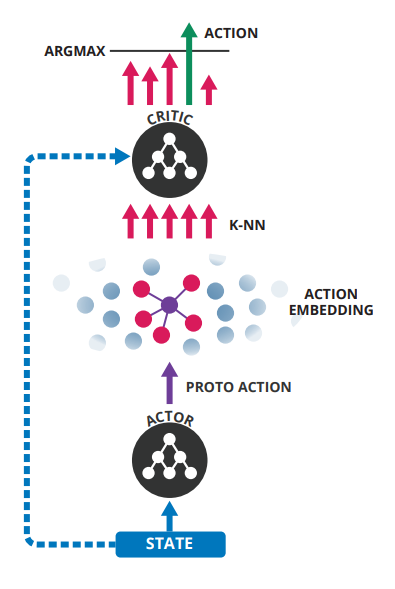
\includegraphics[width=0.4\textwidth]{figures/protoAction.png}
    \caption{Wolpertinger Architecture \cite{protoAction}}
    \label{fig:Wolpertinger_Architecture}
\end{figure}

The idea developed in this paper is to use the continuous action return by the actor of the classical DDPG as a proto-action $\hat{a}$. The authors called this action a proto\-action because this is not the action that the discrete policy will return. Indeed, this proto\-action is likely to not be a valid action ($\hat{a} \notin U$). Therefore, as a first phase, they map from $\hat{a}$ to element(s) in $U$ using $k$-nearest-neighbor ($KNN$) : this algorithm returns the $k$ actions in $U$ that are closest to $\hat{a}$ by $\mathcal{L}2$ distance. To be efficient and scalable, they used the fast library for approximate nearest neighbors (FLANN) developed in the paper \textit{Scalable Nearest Neighbor Algorithms
for High Dimensional Data} \cite{flann}. The approximate $k$-nearest-neighbor will return $k$ potential actions. Then, to choose which one of those actions it is best to return, they will be feeded to the critic (along with the state passed at the input of the actor) such as only the action leading to highest value of the critic will be return by the discrete policy. This second phase is a really important part of their algorithm: it significantly increases the robustness to imperfections in the choice of action representation, and is essential in making their system learn in certain domains. \\

Back on our IDDPG, we straightforwardly apply this concept to our continuous actor to turn it into a discrete one. We called the new class representing this discrete policy \tt{Actor\_discrete\_nn} and it can be found inside the \tt{nn.py} file.

\subsection{Hyperparameters}

{\centering
\begin{minipage}{.6\linewidth}
\begin{table}[H]
    \begin{tabular}{l|l}
        \hline
         Parameter & Value \\
         \hline
         \hline
         \textbf{Shared} & \\
         optimizer & Adam \cite{adam} \\
         learning rate & $3 \cdot 10^{-4}$ \\
         discount factor($\gamma$) & $0.95$ \\
         replay buffer size & $10^6$ \\
         $\tau$ & 0.005 \\
         number of hidden layers (all networks) & 2 \\
         number of hidden neurons per layer & 256 \\
         non-linearity & $ReLU$ \\
         \hline
         \textbf{IDDPG with continuous policy} & \\
         number of samples by minibatch & $256$ \\
         number of steps in the warm up phase & $256$ \\
         \hline
         \textbf{IDDPG with discrete policy} & \\
         number of samples by minibatch & $32$ \\
         number of steps in the warm up phase & $32$ \\
         discrete action space $U$ & \{-1, -0.5, 0, 0.5, 1 \} \\
         number of nearest neighbors return by $KNN$ & 3 \\
         \hline
    \end{tabular}
    \caption{IDDPG Hyperparameters}
    \label{tab:para}
\end{table}
\end{minipage}
\par
} 
\vspace{0.7cm}

Almost all the values of these parameters have been taken from the paper \cite{sac} where it is shown that those values lead to very efficient results. However, as asked, we took $\gamma$ equal to $0.95$. We set the number of steps in the warm up phase equal to the size of the minibatch in order to be able to make the update of the four neural networks directly with minibatch. We have taken a different size of minibatch in function of the policy used to have a good trade-off between training time and efficiency. Indeed, the used of $KNN$ with the discrete policy makes the training a lot slower. This slow computation is also the reason why we choose a value of $k$ equal to $3$ and a discrete action space of only 5 distinct values: it allows a good trade-off between policy quality and speed.

\subsection{Training of IDDPG}


\begin{figure}[H]
    \centering
   % \includegraphics{}
    \caption{Training curves}
    \label{fig:training_IDDPG}
\end{figure}


\subsection{Evaluation}

\subsection{Possible improvements of our approach}

To improve our approach we could implement the full soft actor-critic (SAC) \cite{sac} algorithm. This technique is an off-policy maximum entropy deep reinforcement learning algorithm that has been proven to improve the sample efficiency while increasing the stability and the robustness. Furthermore, the structure of this algorithm is very close to the one of our IDDPG. \\

Another possibility to directly improve the result of IDDPG on the "Inverted Double Pendulum" environment will be to tune the hyperparameters describe in Table~\ref{tab:para}. Indeed, we did not have the time to do an ablation study to find the impact of each parameter and to tune them accordingly. For example, we choose $\mathcal{N}$ to be a Gaussian noise however maybe using an autocorrelated noise \cite{autocorrelated} process to generate temporally correlated
exploration would lead to better results since the inertia presents in the "Inverted Double Pendulum" environment logically injects some correlations. 

\vfill
\bibliographystyle{apacite}
\bibliography{bibli.bib}

\end{document}